\documentclass{beamer}

\mode<presentation>
{\usetheme{boxes}}

\usepackage{times}
\usepackage{graphicx}
\usepackage{hyperref}
\usepackage{listings}
\usepackage{relsize}
\usepackage[T1]{fontenc}

\lstdefinestyle{customc}{
  belowcaptionskip=1\baselineskip,
  breaklines=true,
  frame=L,
  xleftmargin=\parindent,
  language=C,
  showstringspaces=false,
  basicstyle=\footnotesize\ttfamily,
  keywordstyle=\bfseries\color{green!40!black},
  commentstyle=\itshape\color{purple!40!black},
  identifierstyle=\color{blue},
  stringstyle=\color{red},
}
\lstdefinestyle{custombash}{
  belowcaptionskip=1\baselineskip,
  breaklines=true,
  frame=L,
  xleftmargin=\parindent,
  language=bash,
  basicstyle=\footnotesize\ttfamily,
  showstringspaces=false,
  commentstyle=\itshape\color{purple!40!black},
  keywordstyle=\itshape\color{green!40!black},
  identifierstyle=\color{blue},
  stringstyle=\color{orange},
}

\usebackgroundtemplate
{
  \hbox to \paperwidth{\hfil
\includegraphics[opacity=0.3,width=4in,
      height=\paperheight]{wildcat_transparent.jpg}\hfil}
}

\title{PHYS 105 Lecture 2: Variables, Math, and Input/Output}
\author{Tom McClintock \\
	Dept. of Physics\\
	University of Arizona
}
\date{\today}

\begin{document}

\begin{frame}
  \titlepage
\end{frame}

\begin{frame}
  \frametitle{Last Time}
  \begin{itemize}
    \item Logging in to faraday with SSH
    \item Opening programs with emacs
    \item Printing messages with printf()
    \item Compiling and running
    \item Adding comments to code
  \end{itemize}
\end{frame}

\begin{frame}
  \frametitle{This time}
  \begin{itemize}
    \item Optional textbook
    \item Finding your HW grades
    \item More terminal commands
    \item Variables and basic math
    \item I/O from the user
  \end{itemize}
\end{frame}

\begin{frame}
  \frametitle{Textbook - The C Programming Language}
  Our textbook is entitled \textit{The C Programming Language} by
  Kernighan and Ritchie. These two are also the inventors of C.\\
  It is FREE to download online as a pdf. The first link on Google is 
  a download link.\\
  \begin{center}
    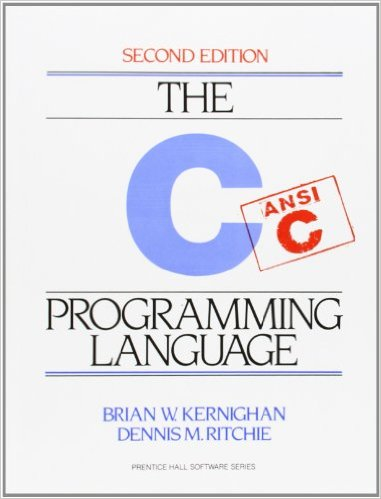
\includegraphics[width=0.3\textwidth]{CPL.jpg}
  \end{center}
\end{frame}

\begin{frame}
  \frametitle{HW Grades and Feedback}
  This information can be found on D2L.\\
  From the D2L homepage, navigate to Dropbox, and then the 
  particular homework (e.g. HW1).\\
  Your number grade is on the right. Click on the speech bubble 
  to see any feedback.
\end{frame}

\begin{frame}
  \frametitle{Terminal Commands Cont.}
  Last time you learned some terminal commands that let you open 
  \textbf{emacs}.\\
  More terminal commands include:
  \begin{itemize}
    \item \textbf{ls} - this stands for ``list''. It shows all files in the 
      current directory (more on that later).
    \item \textbf{history} - this shows a history of all of 
      the commands you have ever issued.
      This is very useful to remind yourself what commands you have done.
    \item \textbf{pwd} - this stands for ``present working directory''. 
      This shows you 
      \textbf{where} in the computer your terminal is located. 
      The default location is 
      ``/home/username/'' where \textit{username} is your username.
    \item \textbf{mkdir} - stands for ``make directory''. 
      Directories are like filing 
      cabinets. They are where you can store programs you make.
    \item \textbf{cd} - stands for ``change directory''. 
      This lets you navigate your terminal throughout different directories.
  \end{itemize}
\end{frame}

\begin{frame}[fragile]
  \frametitle{Making a Directory}
  We are going to create a directory for today's class and work 
  in that today.\\
  Issue the following two commands:
  \begin{lstlisting}[style=custombash]
    mkdir Lecture2
    ls
  \end{lstlisting}
  You should see all of the programs you made last time (hello.c),
  as well as a new directory called Lecture2.
\end{frame}

\begin{frame}[fragile]
  \frametitle{Changing Directories}
  Now you want to \textit{change into} the new directory
  \begin{lstlisting}[style=custombash]
    cd Lecture2
  \end{lstlisting}
  Then try running \textbf{ls} again. You should see nothing there.\\
  Try running \textbf{pwd} and you can see that your terminal is 
  in ``/home/username/Lecture2/''.\\
  You have now \textbf{navigated downwards} into a new directory. 
  In order to navigate 
  \textbf{back up one level} you use \textbf{cd} again with:
  \begin{lstlisting}[style=custombash]
    cd ..
  \end{lstlisting}
  The ``..'' stands for ``up one level''. 
  For the rest of today's lecture work in the directory you have just created.
\end{frame}

\begin{frame}[fragile]
  \frametitle{Variables}
  In the C programming language, information is stored in \textbf{variables}.\\
  Variable names can be whatever you want.\\
  The kinds of variables we will work with for now are integers (\textbf{int}) and
  floating-point variables (\textbf{float}).
  \begin{lstlisting}[style=customc]
    int i = 3;
    int toms_cool_variable_name = 9;
    float a = 64.0;
    float b = 12.7;
  \end{lstlisting}
\end{frame}

\begin{frame}[fragile]
  \frametitle{variables.c}
  In emacs, open up a program called ``variables.c'' with the following command
  \begin{lstlisting}[style=custombash]
    emacs variables.c
  \end{lstlisting}
\end{frame}

\begin{frame}[fragile]
  \frametitle{variables.c}
  \lstinputlisting[style=customc]{variables.c}
  As you can see, variables can be printed in printf() 
  by \textit{passing them in as arguments}.\\
  Integers are printed with a \%i and floats are printed with a \%f.
\end{frame}

\begin{frame}[fragile]
  \frametitle{Save, Compile, and Run}
  Save your program\\
  \vspace{12pt}
  Compile your program with 
  \begin{lstlisting}[style=custombash]
    gcc variables.c -o variables.exe
  \end{lstlisting}
  Then run your program with
  \begin{lstlisting}[style=custombash]
    variables.exe
  \end{lstlisting}
  \vspace{12pt}
  Congrats! You just ran your second program.
\end{frame}

\begin{frame}[fragile]
  \frametitle{Terminology for Variables}
  When a variable is created, we say it is \textbf{declared}
  \begin{lstlisting}[style=customc]
    int i;
  \end{lstlisting}
  The first time a variable is given a value, we say it is \textbf{initialized}
  \begin{lstlisting}[style=customc]
    i = 7;
  \end{lstlisting}
  These two operations don't have to occur at the same time, but a variable \textbf{must}
  be declared before it is used, or else you get an error!\\
  In general, when a variable is given a value we say it is \textbf{assigned} a value
  \begin{lstlisting}[style=customc]
    int i; //the declaration
    i = 7; //first assignment is initialization
    i = 6; //now it is assigned 6
    i = -4; //now it is assigned -4
  \end{lstlisting}
\end{frame}

\begin{frame}[fragile]
  \frametitle{Basic Math}
  We can do math with variables and assign the result to another variable.
  \begin{lstlisting}[style=customc]
    int j = i + 7;
    int k = i * j;
    int l = k / i;
    int m = j - 7;
  \end{lstlisting}
  These are the four basic mathematic operations.\\
  Parentheses work as expected.\\
  We will learn more about math later on.
\end{frame}

\begin{frame}[fragile]
  \frametitle{Input from the User}
  We have already seen that printf() can be used to output text.\\
  What if we want input from the user?\\
  We can use the function scanf().
  \begin{lstlisting}[style=customc]
    int number;
    printf(``Enter a number please:'');
    scanf(``%i'', &number);
  \end{lstlisting}
  We pass scanf() any variable that we want to give input for.\\
  \textbf{Note:} a \& is required when using scanf() for technical reasons.
\end{frame}

\begin{frame}
  \frametitle{squared.c}
  Write this program that takes a number and outputs its square.
  \lstinputlisting[style=customc]{squared.c}
\end{frame}

\begin{frame}[fragile]
  \frametitle{In Class Assignment}
  Write a program that takes a floating point number from the user that represents
  a temperature in degrees Fahrenheit. Store this in a variable called Ftemp, or 
  fahr, or something similar.\\
  Calculate the temperature in degrees Celsuis using the equation
  \begin{equation*}
    C = \frac{5.0}{9.0}(F-32.0)
  \end{equation*}
  Print out the temperature in Celsius to the screen.
\end{frame}

\begin{frame}
  \frametitle{Next time}
  \begin{itemize}
    \item Errors!
    \item If/Else
    \item Blocks \& Scoping
    \item Math library
  \end{itemize}
\end{frame}

\begin{frame}
  \frametitle{HW 2 - two weeks}
  You now have the tools to complete HW 2 which is due in two weeks.\\
  \vspace{12pt}
  Write a program that takes three floats from the user: a length, width, and height of a box.\\
  After taking in the three numbers, calculate the volume of the box and print it out.\\
  Remember to comment your code! The more the better!
\end{frame}


\end{document}